\section{Flexible Mat Prototypes}
\label{sec: Flexible_Mat_Prototypes}
The goal of these prototypes was to create a small silicone mat where the magnet could be suspended in a membrane integrated into the mat itself.
The coil and its heatsink would also be "trapped" inside the mat.
As the mat would be made of silicone, it would allow the device to flex with the flexible coil.
As we can't 3D print silicone we had to create the entire design to be able to make it by silicone casting taking into account all the design limitations of this method.
All the pieces were designed in SolidWorks and then 3D printed to create the molds for the silicone casting. 

% -- Subsection 3.1
\subsection{Design of the membrane}
\label{sec: Design_of_the_membrane}
The design goal for the membrane was to create a structure that could support the magnet \textbf{just enough} to win over its gravitational force so that any other force applied to it on the z-axis would be enough to move it and make it vibrate.
For the membrane design, we decided to use a simple Celtic-cross structure as we described previously in section \ref{sec: Membrane-magnet_system}.
This resulted in a membrane with a central cylindrical chamber used to trap the magnet which is \textbf{suspended} by four parallelepipedal arms.
\begin{figure}[H]
    \centering
    \includegraphics[width=0.7\linewidth]{Chapters/Chapter5/Flexible_Mat_Prototypes/Figures/membrane_v1.png}
    \caption{Membrane top view of the small magnet prototype.}
    \label{fig: Membrane_v1_model}
\end{figure}

\subsubsection{Material stiffness and thickness}
While prototyping we experimented with the same two different silicone materials we described in section \ref{sec: Sleeve_production}.
We quickly realized that the softer silicone was \textbf{too soggy} as the membrane arms would need to be too thick to support the magnet.
We so decided to move forward with only the \textbf{harder silicone} which allowed us to create thinner arms.

\subsubsection{Membrane structure vs magnet dimensions}
The main prototypes we realized were designed with two different N52 cylindrical magnets in mind.
The first one is a small \textbf{10mm} diameter and \textbf{2mm} thick magnet, the second one is a \textbf{15mm} diameter and \textbf{3mm} thick magnet.
The two magnets also have \textbf{very different weights}, the small one weighs \textbf{1.13g} while the big one \textbf{4.03g}.
The first design of the membrane was based on the \textbf{small magnet}, thanks to it being \textbf{lightweight} it could be supported by a membrane with \textbf{very thin arms} (\textbf{0.6mm}) and a width of \textbf{4mm}.
The membrane arms needed also to be \textbf{long enough} to allow the magnet to move freely on the z-axis, so we decided to make them \textbf{4mm} long.
\begin{figure}[H]
    \centering
    \resizebox{0.9\textwidth}{!}{
        \includegraphics{Chapters/Chapter5/Flexible_Mat_Prototypes/Figures/membrane_v1_section.png}
    }
    \caption{Membrane cross-section of the small magnet prototype (t->thickness, L->length).}
    \label{fig: Membrane_v1_section}
\end{figure}

Switching to the big magnet we realized that the membrane arms would need to be \textbf{thicker} to support the magnet, even if we made them wider (\textbf{5mm}).
This was due to the increased weight of the magnet and the increase in the arms' length (now \textbf{5mm}) we needed to make to allow the magnet to move.
To find the new necessary \textbf{minimal thickness} we used the model described in subsection \ref{sec: Membrane_stiffness}.
We set a \textbf{maximum deflection} of \textbf{0.8mm} for the membrane arms and calculated the thickness needed to support the magnet using equations \ref{eq: Beam_deflection} and \ref{eq: Beam_inertia}.
The results showed that the membrane arms would need to be at least \textbf{1.45mm} thick to support the magnet, so we decided to make them \textbf{1.6mm} thick to have a \textbf{safety margin}.

The next problem we encountered arose when we observed that the membrane arms were \textbf{breaking} at the connection with the cylindrical chamber.
This was due to the \textbf{abrupt change of profile} that was causing a stress concentration at that point.
To solve this problem we decided to add a \textbf{small fillet} to the connection between the arms and the chamber.
\begin{figure}[H]
    \centering
    \includegraphics[width=0.9\linewidth]{Chapters/Chapter5/Flexible_Mat_Prototypes/Figures/membrane_v2_section.png}
    \caption{Membrane cross-section of the big magnet prototype.}
    \label{fig: Membrane_v2_section}
\end{figure}

% -- Subsection 3.2
\subsection{Design of the mat}
The mat structure is based on a simple idea but its design was \textbf{quite complex to be realized with silicon casting}. This is mostly due to our goal of integrating the membrane into the mat itself.
This is due to our design goals:
\begin{itemize}
    \item The membrane and magnet need to be \textbf{integrated into the mat} structure.
    \item There needs to be a mechanical way to keep the \textbf{coil} and its \textbf{heatsink} \textbf{steady} inside the silicone structure of the mat, as nothing can be glued to silicone.
    \item We need to create a \textbf{channel} for the magnet chamber to move freely on the z-axis.
    \item The complete structure must be able to \textbf{flex} somewhat.
\end{itemize}

As the silicon sleeve of the previous prototype \ref{sec: Sleeve_production} we opted for a \textbf{two-part mold} to create the mat:
\begin{itemize}
    \begin{samepage}
        \item \textbf{Mold cavity: } The cavity was designed as a \textbf{parallelepipedal} empty box to create a simple external structure for the mat.
        \nopagebreak

        \begin{figure}[H]
            \centering
            \includegraphics[width=0.5\linewidth]{Chapters/Chapter5/Flexible_Mat_Prototypes/Figures/mold_cavity.png}
            \caption{Flexible mat mold cavity}
            \label{fig: mat_mold_cavity}
        \end{figure}
        \nopagebreak

        The purple component in figure \ref{fig: mat_mold_cavity} has four screw holes at the top to screw the \textbf{suspended core} to the cavity.
        The cavity also has a rectangular hole at the bottom where the small component in light blue is inserted.
        This component function is to work as a \textbf{pedestal} for the magnet, its exact function will be explained in the next section.
        \nopagebreak

        Through both components are carved four holes, these are used to allow the \textbf{excess silicone} of the casting process to \textbf{flow out} of the cavity.
        \nopagebreak

        The purple part needs to be 3D-printed in a flexible material to allow the mat to be \textbf{easily removed} from the cavity, in our case we used \textbf{TPU}.        
    \end{samepage}
    

    \item \textbf{Mold core: } The core is composed of multiple components that are inserted into the cavity to create the internal structure of the mat.
    \begin{figure} %TODO: Fix dimensions of the compose
        \centering
        \begin{subfigure}[b]{0.6\textwidth}
            \begin{subfigure}[b]{0.475\textwidth}
                \centering
                \includegraphics[width = 1\linewidth]{Chapters/Chapter5/Flexible_Mat_Prototypes/Figures/mold_core_exploded_top.PNG}
                \caption{Exploded top view of the mold core.}
            \end{subfigure}
            \hfill
            \begin{subfigure}[b]{0.475\textwidth}
                \centering
                \includegraphics[width = 1\linewidth]{Chapters/Chapter5/Flexible_Mat_Prototypes/Figures/mold_core_exploded_btm.PNG}
                \caption{Exploded bottom view of the mold core.}            
            \end{subfigure}
            \vskip\baselineskip
            \begin{subfigure}[b]{0.475\textwidth}
                \centering
                \includegraphics[width = 1\linewidth]{Chapters/Chapter5/Flexible_Mat_Prototypes/Figures/mold_core_top.PNG}
                \caption{Assembled top view of the mold core.}
            \end{subfigure}
            \hfill
            \begin{subfigure}[b]{0.475\textwidth}
                \centering
                \includegraphics[width = 1\linewidth]{Chapters/Chapter5/Flexible_Mat_Prototypes/Figures/mold_core_btm.PNG}
                \caption{Assembled bottom view of the mold core.}
            \end{subfigure}
        \end{subfigure}
        \caption{Assembly of the mold core}
        \label{fig: mat_mold_core}
    \end{figure}

    In figure \ref{fig: mat_mold_core} we can see all the components of the core, which are:
    \begin{itemize}
        \item \textbf{Mold core center } (in light blue) \textbf{: } This is the central component of the core, it is used to create the \textbf{coil membrane} and the \textbf{channel} for the magnet chamber to move.
        \item \textbf{Coil trap} (in red) \textbf{: } This is the structure that will house the \textbf{coil} and its \textbf{heatsink} and the only part of the core that will remain inside the mat.
        \item \textbf{Mold core cap } (in yellow) \textbf{: } This component is used to \textbf{keep the coil trap in place} and to prevent the silicone from \textbf{entering the coil trap}.
        \item \textbf{Mold core - cavity bridge } (in pink) \textbf{: } This part screws into the core and the cavity to keep the core \textbf{suspended} in the cavity.
    \end {itemize}
    
\end{itemize}

\subsubsection{Magnet chamber and membrane}
To create the membrane and trap the magnet inside its chamber we needed a way to allow the silicone to \textbf{flow all around} the magnet.
\begin{figure}[H]
    \centering
    \begin{subfigure}[b]{0.8\linewidth}
        \begin{subfigure}[b]{0.475\textwidth}
            \centering
            \includegraphics[width=\linewidth]{Chapters/Chapter5/Flexible_Mat_Prototypes/Figures/mat_mold_core_center_top.PNG}
            \caption{Mold core center top view.}
            \label{fig: mat_mold_core_center_top}
        \end{subfigure}
        \hfill
        \begin{subfigure}[b]{0.475\textwidth}
            \centering
            \includegraphics[width=\linewidth]{Chapters/Chapter5/Flexible_Mat_Prototypes/Figures/mat_mold_core_center_btm.PNG}
            \caption{Mold core center bottom view.}
            \label{fig: mat_mold_core_center_btm}
        \end{subfigure}
    \end{subfigure}    
    \caption{Mold core center.}
    \label{fig: mat_mold_core_center}
\end{figure}

To create the upper part of the chamber we modeled the mold core center to have a cylindrical hole in its center, deep and large enough to create a \textbf{silicone wall around the magnet} with a lateral thickness of \textbf{0.5mm} and a bottom thickness of \textbf{1.2mm}.

To cast the upper part of the chamber we created a \textbf{pedestal} (the light blue component in figure \ref{fig: mat_mold_cavity}) for the magnet to rest on, the pedestal is a simple rectangular structure with a small circular bump at its center where the magnet is \textbf{glued} on.
When the silicone is set the pedestal can be \textbf{removed} and the magnet will be trapped inside the chamber by an \textbf{upper silicone ceiling} of thickness \textbf{0.6mm}.
The \textbf{curved parts} and the \textbf{square holes} we can see in figure \ref{fig: mat_mold_core_center} are used to create the \textbf{membrane arms}.

The part used to create the channel is composed of three \textbf{different-sized cylinders}, the \textbf{first one} (the largest) is used to create the \textbf{space for the membrane arms to flex}, the \textbf{second one} is used to create the \textbf{channel itself} and the \textbf{third} \textbf{one} is used as a \textbf{support} for the coil trap and cap to \textbf{embed} them.

On the top, the center component presents four holes that are used to \textbf{screw it} onto the cap and one \textbf{larger central one} that reaches through up to the \textbf{magnet surface} which is used to pour the silicone into the chamber.

When the silicone is set the core center would remain \textbf{stuck into the mat} as it is too complex to be removed without damaging the mat itself.
To solve this problem we decided to create the core center in a material that could be easily \textbf{dissolved} in water.
This material is called \textbf{BVOH} and is a \textbf{water-soluble} filament that can be used as a support material for 3D printing.
To speed up the \textbf{dissolution process} we decided to print the core center with \textbf{low infill} and shave some material off the smallest cylinder to allow the water to reach the BVOH more easily.

\subsubsection{Distance magnet-coil}
The middle cylinder is what dictates the \textbf{distance} between the \textbf{magnet} and the \textbf{coil}.
This distance is crucial as it will determine the \textbf{strength of the magnetic field} that will reach the magnet.
After multiple prototypes, we landed on a distance of \textbf{3.5mm} between the magnet and the coil.
In theory, the distance could be lower but we had to take into account the \textbf{flexing of the membrane due to the pressure} on it generated by the finger grasping the device.

\subsubsection{Coil trap}
This component has two functions, the first one is to \textbf{house the coil} and its heatsink and the second one is to \textbf{trap the coil} mechanically inside the mat.
Our main design limitations were that we \textbf{couldn't glue} the trap to the mat and that the trap needed to be able to \textbf{flex} with the mat and coil.

\begin{figure}[H]
    \centering
    \begin{subfigure}[b]{0.8\linewidth}
        \begin{subfigure}[b]{0.475\textwidth}
            \centering
            \includegraphics[width=\linewidth]{Chapters/Chapter5/Flexible_Mat_Prototypes/Figures/coil_trap_expl.png}
            \caption{Coil trap exploded view.}
            \label{fig: coil_trap_expl}
        \end{subfigure}
        \hfill
        \begin{subfigure}[b]{0.475\textwidth}
            \centering
            \includegraphics[width=\linewidth]{Chapters/Chapter5/Flexible_Mat_Prototypes/Figures/coil_trap_closed.png}
            \caption{Coil trap with coil closed view.}
            \label{fig: coil_trap_closed}
        \end{subfigure}
    \end{subfigure}   
    \caption{Coil trap model.}
    \label{fig: mat_mold_core_trap}
\end{figure}

The design we came up its a thin \textbf{square structure} with a small higher \textbf{border} where the coil is positioned (the lower part in figure \ref{fig: mat_mold_core_trap}).
The coil is then covered by a \textbf{thin square plate} that is screwed to the trap (the higher part in figure \ref{fig: mat_mold_core_trap}).
On the side of this square, we have four \textbf{thin fins} that will \textbf{remain inside the silicone structure} of the mat, mechanically \textbf{blocking the trap inside}.
\begin{figure}[H]
    \centering
    \includegraphics[width = 0.7\linewidth]{Chapters/Chapter5/Flexible_Mat_Prototypes/Figures/coil_trap_in_mat.png}
    \caption{Coil trap placed inside the mat.}
    \label{fig: coil_trap_in_mat}
\end{figure}
As the coil trap is very thin and it's printed in \textbf{TPU} it can easily \textbf{flex with the mat and the coil}.

\subsubsection{Production method}
To create a new mat various steps need to be followed:
\begin{itemize}
    \item \textbf{Components printing: } All the components of the core and the cavity need to be printed.
    \item \textbf{Cavity assembling: } We first need to \textbf{glue the magnet to the pedestal} and then place it inside the hole at the bottom of the big part.
    \item \textbf{Core assembling: } We start by placing the bottom part of the coil trap on the smallest cylinder of the core center, then we screw the mold core cap and bridge to the core center and finally we screw the bridge to the cavity.
    \item \textbf{Silicone casting: } We \textbf{mix the silicone} and \textbf{pour it} first into the \textbf{big hole on top of the cap} with a syringe until the chamber is filled, we can notice when it's full by observing the \textbf{holes at the bottom of the cavity} and the membrane holes on the core center.
    We then pour the rest of the silicone into the cavity until the silicone \textbf{covers the coil trap fins}.
    \item \textbf{Removing the mat from the mold: } After the silicone is set we can remove the mat from the mold by unscrewing the bridge and pulling it out. Now we can also remove the pedestal and core cap.
    \item \textbf{Removing the core center: } We then place the mat in a container filled with water and let it \textbf{dissolve} the core center.
    \item \textbf{Finalizing the mat: } After the core center is dissolved we can place the coil with its heatsink inside the trap and screw the cover on.
\end{itemize}
Different prototypes required some different \textbf{additional clean-up} steps to remove some silicone excess.

\begin{figure}[H]
    \centering
    \begin{subfigure}[b]{0.475\textwidth}
        \centering
        \includegraphics[width = 1\linewidth]{Chapters/Chapter5/Flexible_Mat_Prototypes/Figures/mold_complete.png}
        \caption{View of the complete mold.}
        \label{fig: mat_v1}
    \end{subfigure}
    \hfill
    \begin{subfigure}[b]{0.475\textwidth}
        \centering
        \includegraphics[width = 1\linewidth]{Chapters/Chapter5/Flexible_Mat_Prototypes/Figures/mold_complete_exploded.png}
        \caption{Exploded view of the complete mold.}
        \label{fig: mold_v1}
    \end{subfigure}
    \caption{Complete mold for the mat.}
\end{figure}

% -- Subsection 3.3
\subsection{Design faults and problems}

\subsubsection{Membrane fragility}
As we previously touched on in paragraph \ref{sec: Design_of_the_membrane}, the membrane arms tend to break at the connection with the cylindrical chamber.
This is due to the abrupt change of profile that causes a stress concentration at that point.
This problem was especially noticeable during testing, as we had to remove the magnet from the chamber multiple times damaging the structure of the membrane.
Adding some fillets to the connection between the arms and the chamber helped to solve this problem, but it didn't eliminate it.
The good thing is that the membrane is easily fixable by adding very small amounts of silicone to the broken parts as glue and letting it cure.

\subsubsection{Overall system flexibility}
In the case of the small magnet, this design resulted in a pretty flexible device that could be bent a fair amount in all directions.
\begin{figure}
    \centering
    \begin{subfigure}[b]{0.475\textwidth}
        \centering
        \resizebox{\textwidth}{!}{
            \includegraphics{Chapters/Chapter5/Flexible_Mat_Prototypes/Figures/flexing_mat_top.png}
        }        
    \end{subfigure}
    \hfill
    \begin{subfigure}[b]{0.475\textwidth}  
        \centering 
        \resizebox{\textwidth}{!}{
            \includegraphics{Chapters/Chapter5/Flexible_Mat_Prototypes/Figures/flexing_mat_btm.png}
        }
    \end{subfigure}
    \caption{Flexible mat prototype bending.}
    \label{fig: Flexible_mat_bending}
\end{figure}

Meanwhile, in the case of the big magnet, the mat was also pretty flexible but the magnet with its size impeded the structure from bending as much as the small magnet version.

\subsubsection{Coil trap design faults}
The main problem with the coil trap design was that screwing the two parts together is not reliable.
As the two parts are connected by screws in only four points they tend to separate when the mat is bent.
This is because the lower part follows the bending of the mat through its fins, these fins are not directly connected to the upper part.

\begin{figure}
    \centering
    \resizebox{0.9\textwidth}{!}{
        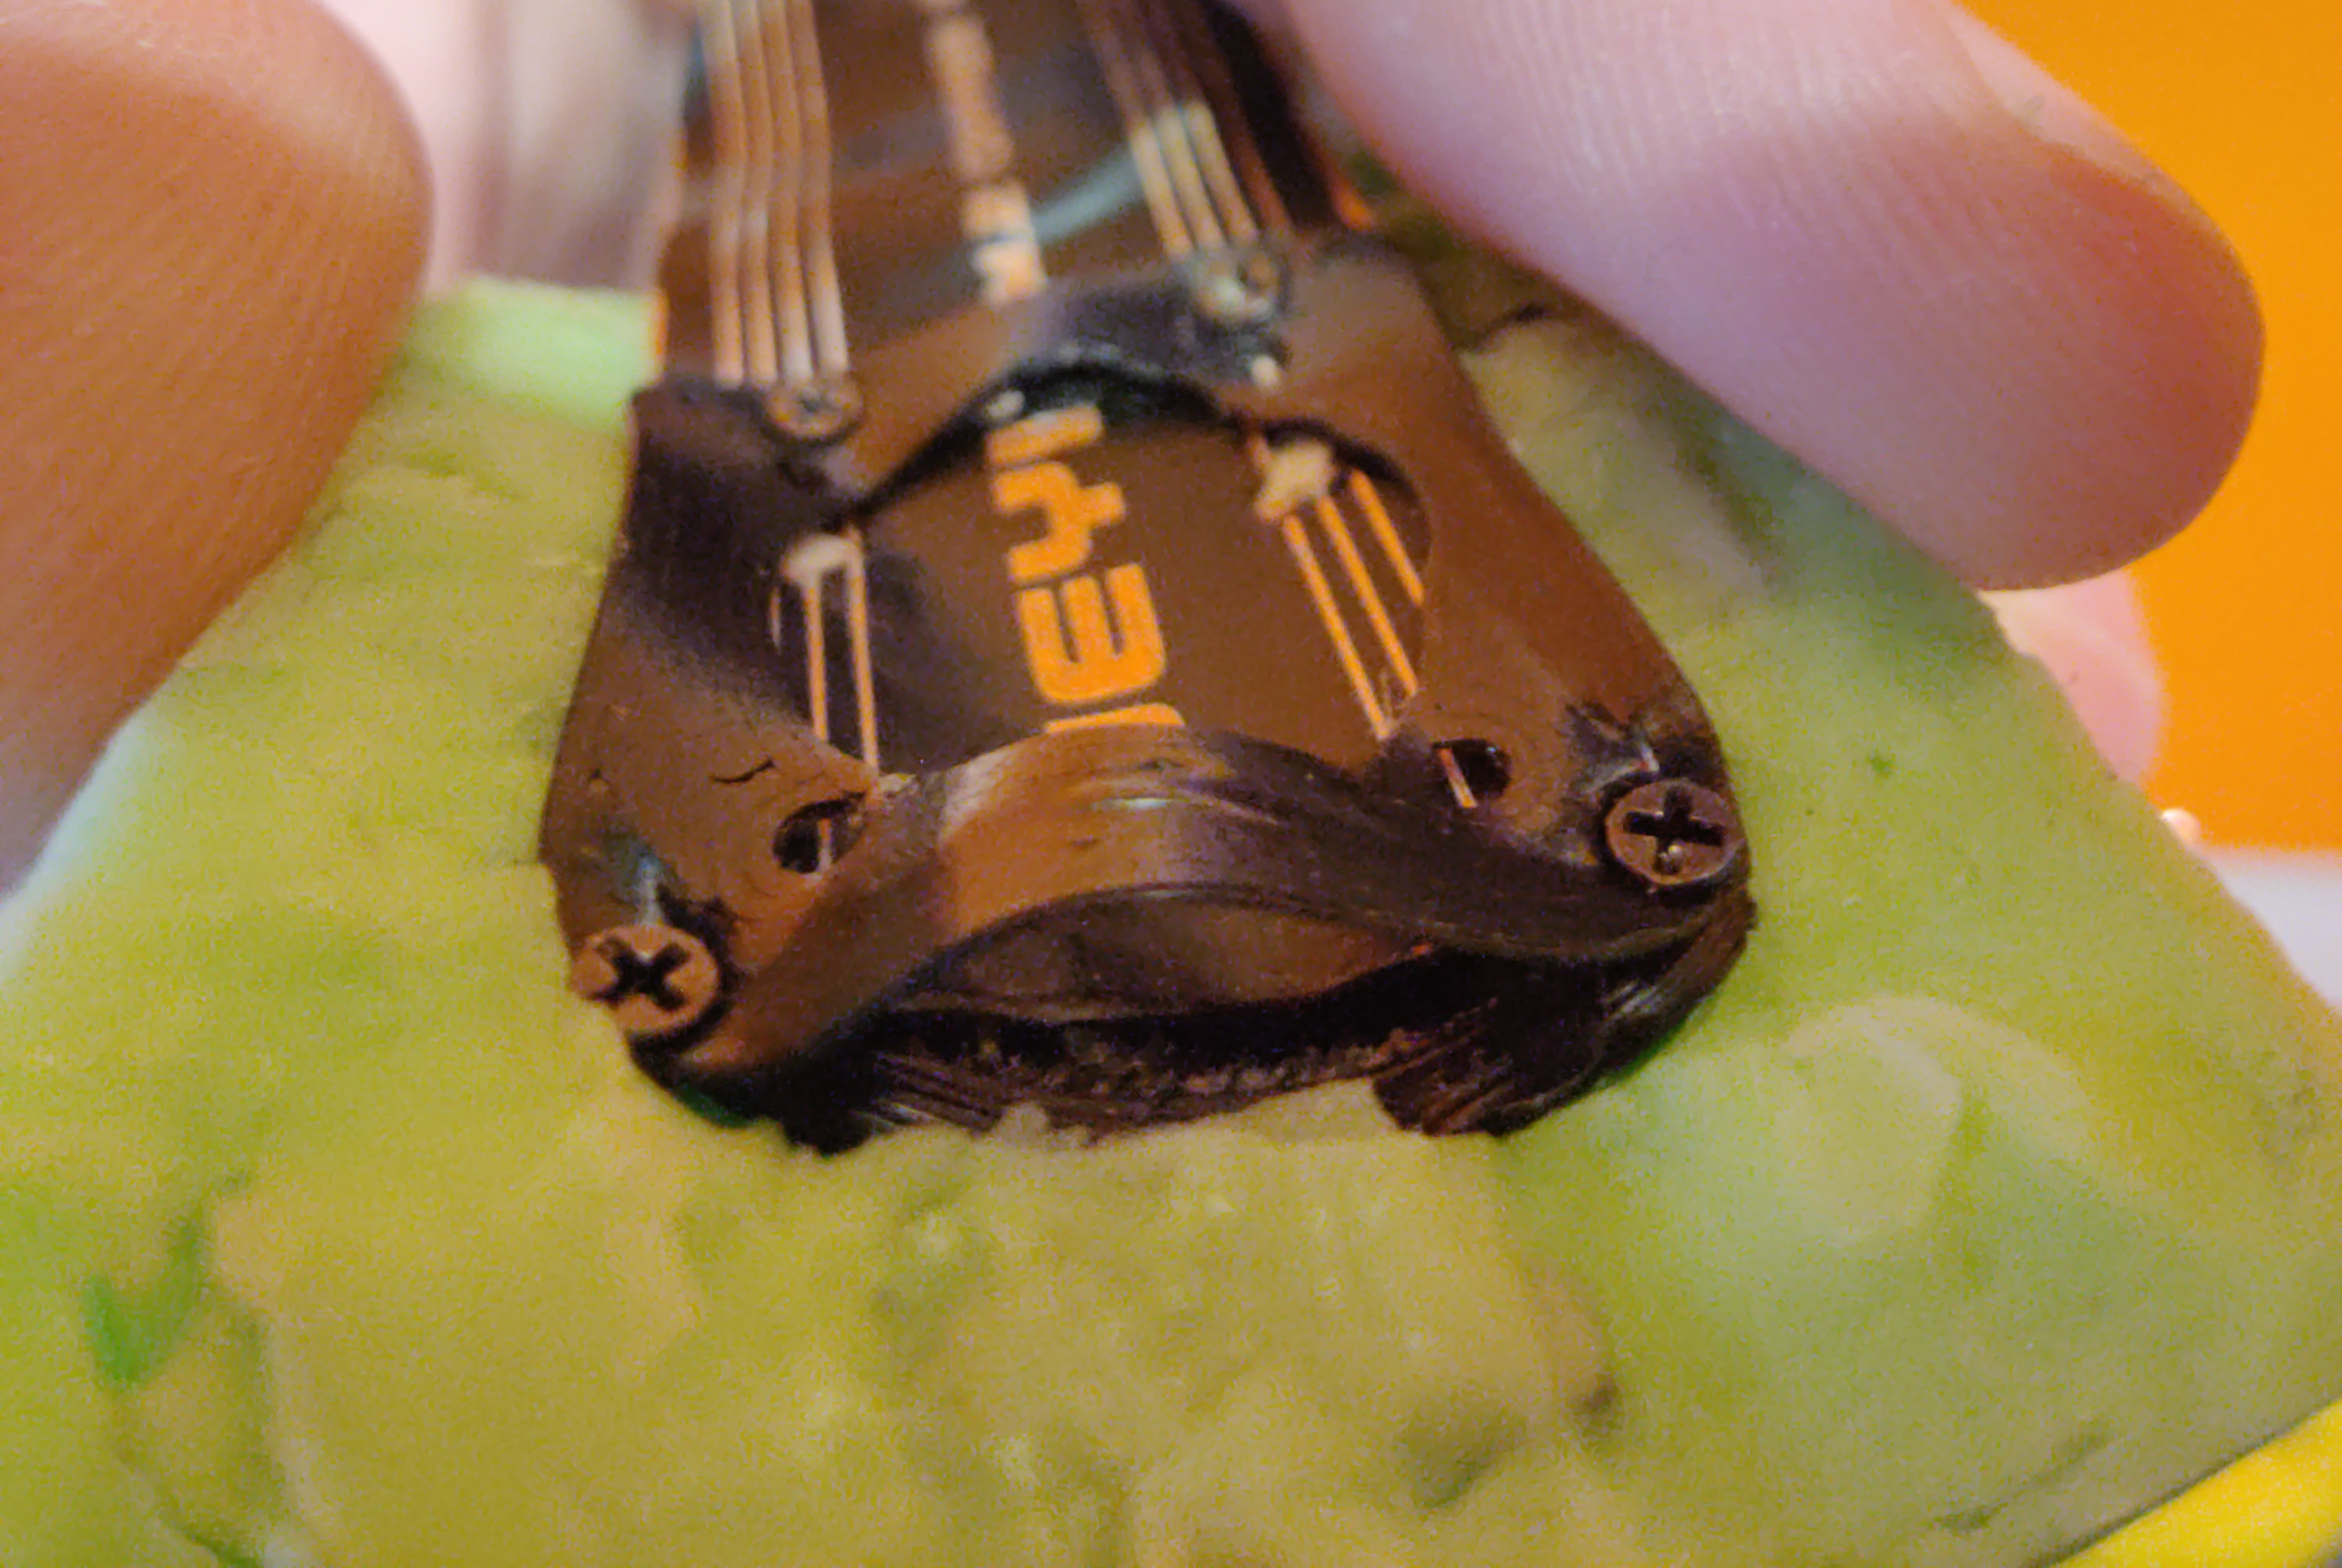
\includegraphics{Chapters/Chapter5/Flexible_Mat_Prototypes/Figures/coil_trap_separating.png}
    }
    \caption{Coil trap separating when the mat is bent.}
    \label{fig: Coil_trap_separating}
\end{figure}